\begin{figure}[htbp]
\centering
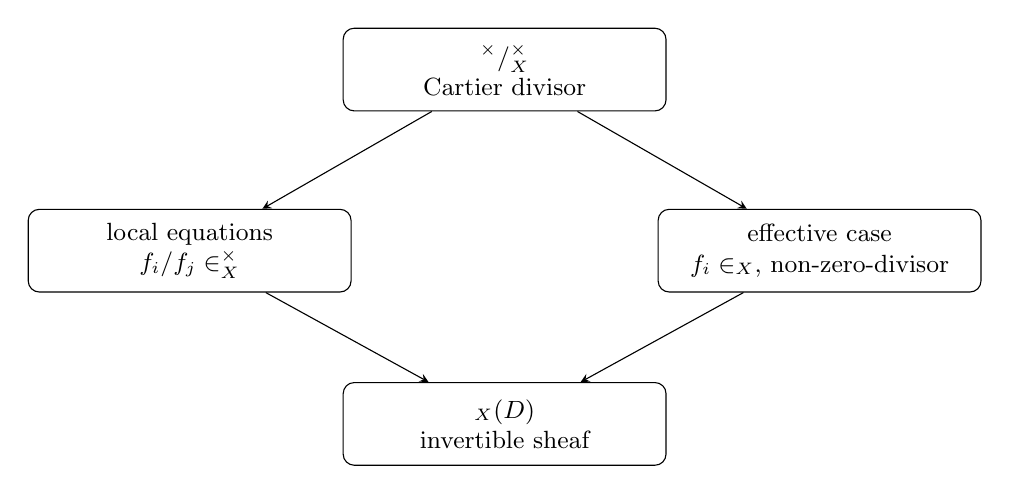
\begin{tikzpicture}[>=stealth,every node/.style={font=\small}]
\node[draw,rounded corners,minimum width=4.1cm,minimum height=1.05cm,align=center] (q) at (0,1.7) {$\KX^\times/\OO_X^\times$\\Cartier divisor};
\node[draw,rounded corners,minimum width=4.1cm,minimum height=1.05cm,align=center] (l) at (-4,-0.6) {local equations\\$f_i/f_j\in\OO_X^\times$};
\node[draw,rounded corners,minimum width=4.1cm,minimum height=1.05cm,align=center] (e) at (4,-0.6) {effective case\\$f_i\in\OO_X$, non-zero-divisor};
\node[draw,rounded corners,minimum width=4.1cm,minimum height=1.05cm,align=center] (b) at (0,-2.8) {$\OO_X(D)$\\invertible sheaf};
\draw[->] (q)--(l);
\draw[->] (q)--(e);
\draw[->] (l)--(b);
\draw[->] (e)--(b);
\end{tikzpicture}
\caption{Cartier divisors connect local rational equations, effective locally principal subschemes, and invertible sheaves.}
\label{fig:vi40-roadmap}
\end{figure}
